\section{Ανάπτυξη Εφαρμογών}
\label{sec:development}

Η παρούσα παράγραφος περιγράφει την διαδικασία που πρέπει να ακολουθηθεί για να αναπτύξει κάποιος μια εφαρμογή η οποία θα προσαρτηθεί πάνω στον καθρέφτη. Η οργάνωση του συστήματος έχει γίνει με την χρήση των κλάσεων kivy.uix.screenmanager.ScreenManager και kivy.uix.screenmanager.Screen. Τα σημεία που πρέπει να προσέξει κάποιος για να προσαρτήσει την δική του εφαρμογή είναι στην δομή των φακέλων του κώδικα, στην ορθή ανάγνωση του Widget από το λειτουργικό του καθρέφτη, οι σωστή δομή των ρυθμίσεων της προσαρτούμενης εφαρμογής και τέλος οι φωνητικές εντολές που θα είναι διαθέσιμες για τον χρήστη.

\subsection{Δομή Φακέλων}
Η δομή που έχει ο κώδικας του καθρέφτη φαίνεται στο παρακάτω δέντρο.
\\

\dirtree{%
	.1 SmartMirror.
	.2 smartmirror.py.
	.2 smartmirror.kv.
	.2 mirror\_settings.py.
	.2 modules/.
	.3 action.py.
	.3 basedir.py.
	.3 bot.py.
	.3 controller.py.
	.3 speech.py.
	.2 widgets/.
	.3 clock/.
	.3 exercisor/.
	.3 weather/.
}

Οποιαδήποτε καινούργια εφαρμογή αναπτύσει ο χρήστης πρέπει να μπει κάτω από τον φάκελο widgets με την παρακάτω δομή. \\

\dirtree{%
	.1 widgets/.
	.2 <widget\_name>/.
	.3 <widget\_name>.py.
	.3 <widget\_name>.kv.
	.3 settings.json.
}

Με την παραπάνω οργάνωση το λειτουργικό είναι σε θέση να βρει αυτόματα και να προσαρτήσει την εφαρμογή.

\subsection{Εγκατάσταση Οθόνης}
Η γενική οργάνωση του καθρέφτη όσον αφορά την λογική των εξωτερικών εφαρμογών φαίνεται στο Σχήμα \ref{fig:widget_organization}. Η κλάση MainPage είναι ένας ScreenManager ο οποίος διαβάζει όλες τις οθόνες που βρίσκονται στον φάκελο widgets/ και τις προσαρτίζει σε αυτόν.

\begin{figure}[h]
	\centering
	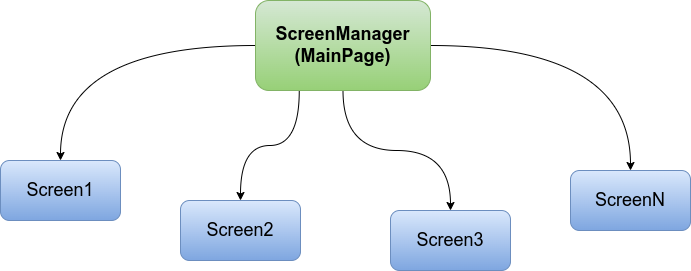
\includegraphics[scale=0.7]{images/chapter6/widget_organization.png}
	\caption{Αναπαράσταση δομής του καθρέφτη}
	\label{fig:widget_organization}
\end{figure}

Προκειμένου να γίνει η προσάρτηση, κάθε widget πρέπει να ορίσει μία συνάρτηση install(manager) η οποία καλεί την εντολή \texttt{manager.add\_widget(<Screen>)}. Κατά την εκκίνηση της εφαρμογής η κλάση MainPage καλεί τις συναρτήσεις install του κάθε widget και έτσι προσθέτει τις συγκεκριμένες οθόνες.

\subsection{Ρυθμίσεις}
Για την ανάγνωση των ρυθμίσεων της εφαρμογής απαιτείται η δημιουργία ενός αρχείου με όνομα settings.json το οποίο θα έχει 2 κλειδιά: το "default\_json" και το "settings\_json". Στο πρώτο κλειδί θα ανατεθεί ένα αντικείμενο που ορίζει τις προκαθορισμένες τιμές που θα έχουν οι ρυθμίσεις, ενώ το δεύτερο κλειδί περιέχει μία λίστα με όλες τις ρυθμίσεις, τα ονόματά τους, τον τύπου τους αλλά και την προκαθορισμένη τιμή τους. Για την καλύτερη κατανόηση παρατίθεται παρακάτω ένα παράδειγμα του αρχείου ρυθμίσεων του Widget Weather. 

\begin{lstlisting}
{
	"default_json": {
		"api_key": "API_KEY",
		"city_id": "CITY_ID",
		"city_name": "CITY_NAME",
		"update_interval": 1800
	},
	"settings_json": [
		{
			"type": "title",
			"title": "Weather"
		},
		{
			"type": "string",
			"title": "API KEY",
			"desc": "Openweathermap API key",
			"section": "weather",
			"key": "api_key"
		},
		{
			"type": "string",
			"title": "City Id",
			"desc": "Openweathermap City's id",
			"section": "weather",
			"key": "city_id"
		},
		{
			"type": "string",
			"title": "City Name",
			"desc": "Openweathermap City's name",
			"section": "weather",
			"key": "city_name"
		},
		{
			"type": "numeric",
			"title": "Update Interval",
			"desc": "How often to update the weather in seconds",
			"section": "weather",
			"key": "update_interval"
		}
	]
}
\end{lstlisting}

Τέλος, η εφαρμογή πρέπει να ορίσει και μία συνάρτηση με όνομα "update\_config" η οποία θα εκτελείται κάθε φορά που γίνεται ανανέωση των ρυθμίσεων προκειμένου να ενημερωθούν οι τιμές των μεταβλητών του Widget. Σε αυτήν την περίπτωση κανείς μπορεί να ανατρέξει στο αρχείο "weather.py" του Widget Weather για ένα παράδειγμα ανάγνωσης ρυθμίσεων μέσω του Kivy και υλοποίηση της συνάρτησης "update\_config".

\subsection{Φωνητικές Εντολές}
Για τον καθορισμό των διαθέσιμων εντολών που παρέχει η εφαρμογή απαιτείται η δημιουργία μιας συνάρτησης με όνομα "subscribe" η οποία επιστρέφει ένα dictionary το οποίο κάνει map τις προθέσεις σε συναρτήσεις που θα κληθούν. Ένα παράδειγμα των διαθέσιμων εντολών του Widget Weather φαίνεται παρακάτω

\begin{lstlisting}
	{
		"request_location": self.request_location,
		"request_hour": self.request_hour,
		"request_day": self.request_day
	}
\end{lstlisting}

Το παραπάνω dictionary υποδεικνύει τρεις εντολές, ανάλογα με την πρόθεση που θα αναγνωρίσει το Wit.ai

Ο χρήστης που αναπτύσσει την εφαρμογή είναι υπεύθυνος να εκπαιδεύσει το Wit.ai με τα δικά του δεδομένα στις δικές τους εντολές και επομένως Θα χρειαστεί να συνδεθεί στην πλατφόρμα στο \href{https://wit.ai}{https://wit.ai}. Ένα βασικό πακέτο εντολών είναι διαθέσιμο στον φάκελο assets/ το οποίο θα μπορεί να εισαχθεί απευθείας στο wit και από εκεί να επεκταθεί ανάλογα τις ανάγκες του χρήστη.